\documentclass{article}
\usepackage{amsmath}
\usepackage{geometry}
\usepackage{float}
\geometry{a4paper, left=2cm, right=2cm, top=2.54cm, bottom=2.54cm}
\usepackage{indentfirst}
\usepackage{enumitem}
\usepackage{bm}
\usepackage[hidelinks]{hyperref}

% 段落間距  (begin doc 才設定)
\usepackage{parskip}
    % 普通文字,行距
    \usepackage[onehalfspacing]{setspace}
    
\usepackage{tabularx}

\usepackage{fontspec,xltxtra,xunicode}

\usepackage{titlesec}

\def\Large{\fontsize{18}{10}\selectfont}
\def\huge{\fontsize{26}{10}\selectfont}
\def\Huge{\fontsize{36}{30}\selectfont}

\titleformat{\section}
  {\fontsize{16pt}{15}\bfseries}
  {\selectfont\thesection.}
  {0.5em}
  {}

\titleformat{\subsection}
  {\fontsize{14pt}{15}\bfseries}
  {\selectfont\thesubsection.}
  {0.5em}
  {}


\usepackage{xeCJK}
\setCJKmainfont[AutoFakeBold=3]{DFKai-SB} %设置中文字体\XeTeXlinebreaklocale “zh”\XeTeXlinebreakskip = 0pt plus 1pt minus 0.1pt %文章内中文自动换行


\usepackage{minted}
\setminted{
baselinestretch=1,
fontsize=\small,
python3=true,
style = tango,
}


\usepackage{caption}
\newenvironment{code}{\captionsetup{type=listing, font=large}}{}

\captionsetup{font=large}



\usepackage{longtable}
\usepackage{array}
\usepackage{makecell}
\renewcommand{\arraystretch}{1.2}

% % 首行縮排
% \usepackage{indentfirst}
% % 首行縮排距離
% \setlength\parindent{28pt}

\renewcommand{\figurename}{Fig.}

\setmainfont{Times New Roman}

\title{\textbf{{\huge HW4 - TCAM Operations} \\ 記憶體積體電路\ Memory\ Circuit\ Design}}
\author{{\Large\textbf{ 電機4A\quad 109501201\quad 陳緯亭}}}
\date{\Large{\today}} 



\begin{document}

% 首行縮排距離
\setlength\parindent{28pt}

% 段落後間距
\setlength\parskip{14pt}

\newcolumntype{L}[1]{>{\raggedright\let\newline\\\arraybackslash\hspace{0pt}}m{#1}}
\newcolumntype{C}[1]{>{\centering\let\newline\\\arraybackslash\hspace{0pt}}m{#1}}
\newcolumntype{R}[1]{>{\raggedleft\let\newline\\\arraybackslash\hspace{0pt}}m{#1}}


\maketitle
\vspace*{-0.5cm}

\fontsize{12pt}{1.5em}

\selectfont

\section{NAND-type TCAM}

$\bullet$ Store Mode: WL 提升至 $V_{DD}$。可以寫入 $\rm BL/SL$ 的值到 $Q_i$ , $\rm \overline{BL}/\overline{SL}$ 的值到 $\rm \overline{Q_i}$。在下方電路中,則會寫入 $\rm DL$ 的值到 $Q_j$,$\rm \overline{DL}$ 的值到 $\overline{Q_j}$。

$\bullet$ Search Mode: 當 $Q_j = V_{DD},\ \overline{Q_j} = 0$ ,此為 Don't care mode。不管 $Q_i(\overline{Q_i})$ 和 $\rm SL(\overline{SL})$ 有沒有匹配。 ML 都 match (0(M))。反之,當 $Q_j = 0,\ \overline{Q_j} = V_{DD}$ ,此為 Care mode,匹配資訊在下方。

\begin{table}[H]
  \centering
  \begin{tabular}{ccccc}
  $Q_i$ & $\overline{Q_i}$ & $\rm SL$ & $\rm \overline{SL}$ & ML \\
  0  & 1     & 0  & 1     & 0(M) \\
  1  & 0     & 1  & 0     & 0(M) \\
  0  & 1     & 1  & 0     & 1(MM) \\
  1  & 0     & 0  & 1     & 1(MM)
  \end{tabular}
  \end{table}

\begin{figure}[H]
\centering
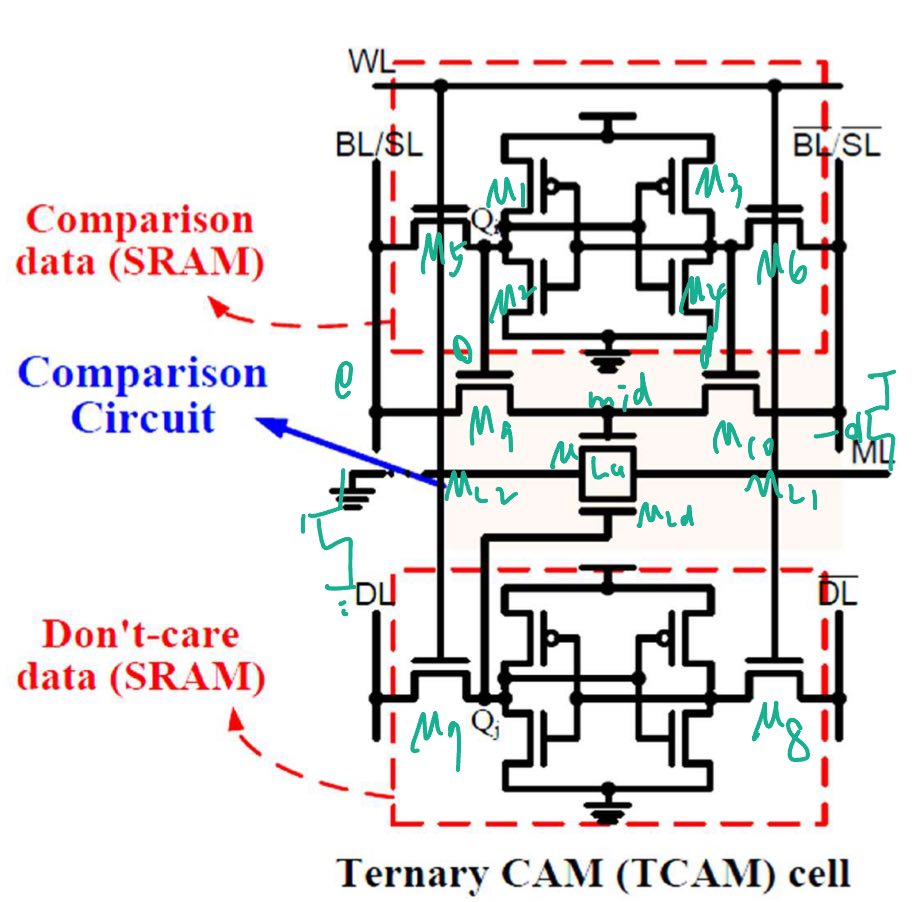
\includegraphics[width=0.5\linewidth]{./img/2023-12-14-00-36-19.png}
\caption{NAND-type Circuit}
\end{figure}


\subsection{Store Mode}

WL 電壓提升至 $V_{DD}$為 logic-1, M5 和 M6 打開,即可用 $\rm BL$ 和 $\rm \overline{BL}$ 寫入資料到 $Q_i$ 和 $\overline{Q_i}$。圖上方的 w0 為寫入 $Q_i = 0$, $\overline{Q_i} = 1$, w1 為寫入 $Q_i = 1$, $\overline{Q_i} = 0$。

\vspace*{-1em}

\begin{figure}[H]
\centering
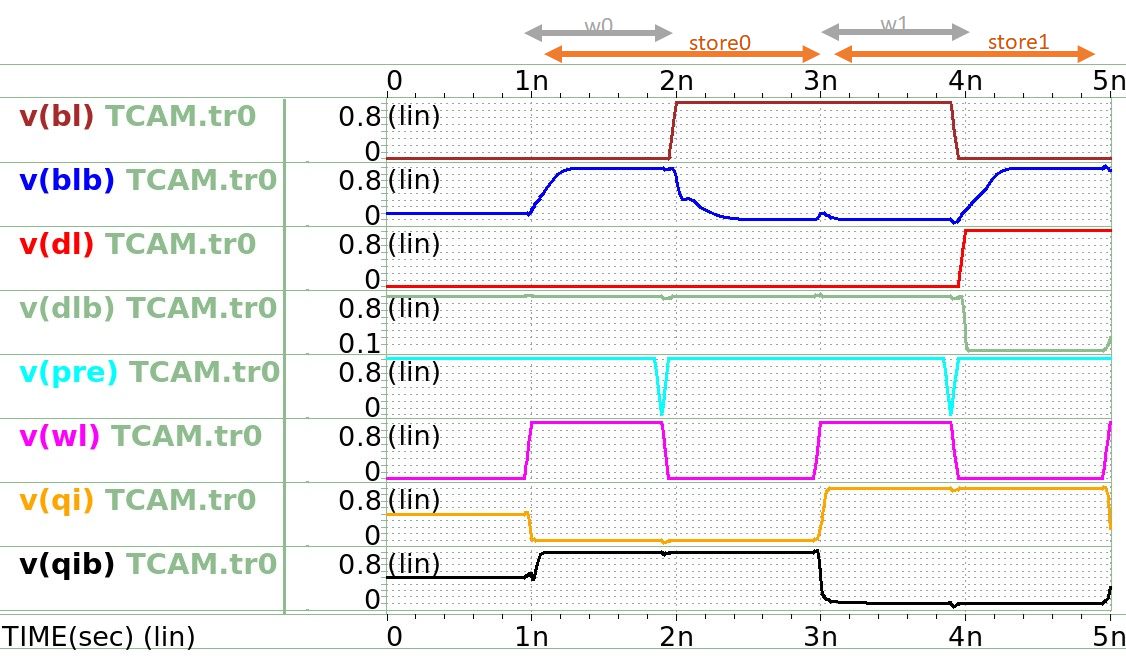
\includegraphics[width=0.8\linewidth]{./img/2023-12-13-23-20-15.png}
\end{figure}

\subsection{Search Mode - Care mode}

在 Care mode 下, $\rm DL$ 和 $\rm \overline{DL}$ 須分別寫入 $0$ 和 $V_{DD}$ 到 $Q_j$ 和 $\overline{Q_j}$,以確保接到 ML 那顆 nMOS 是關閉的。w為寫入,s為搜索資料。match (M) 為 0,mismatch (MM) 為 1。

\begin{figure}[H]
\centering
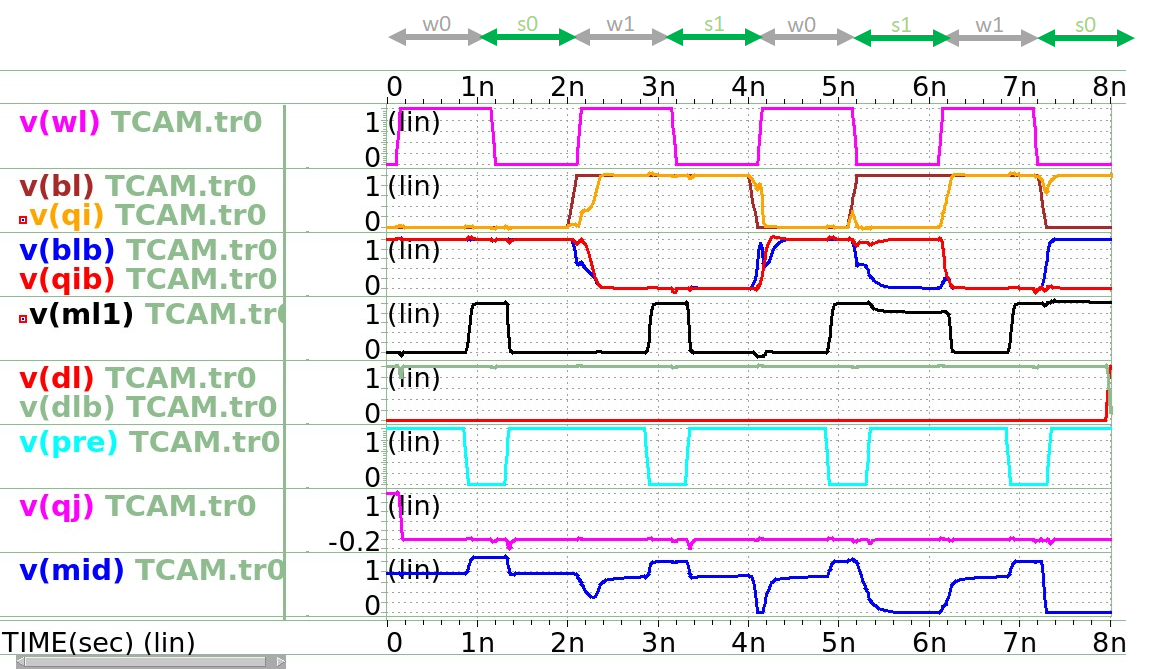
\includegraphics[width=\linewidth]{./img/2023-12-14-00-13-55.png}
\end{figure}

\subsection{Search Mode - Don't care mode}

在 Don't Care mode 下, $\rm DL$ 和 $\rm \overline{DL}$ 須分別寫入 $V_{DD}$ 和 $V_{0}$ 到 $Q_j$ 和 $\overline{Q_j}$,以確保接到 ML 那顆 nMOS 是開啟的。w為寫入,s為搜索資料。

\begin{table}[H]
  \centering
  \begin{tabular}{ccccc}
  $Q_i$ & $\overline{Q_i}$ & $\rm SL$ & $\rm \overline{SL}$ & ML \\
  0  & 1     & 0  & 1     & 0(M) \\
  1  & 0     & 1  & 0     & 0(M) \\
  0  & 1     & 1  & 0     & 0(M) \\
  1  & 0     & 0  & 1     & 0(M)
  \end{tabular}
  \end{table}

\begin{figure}[H]
\centering
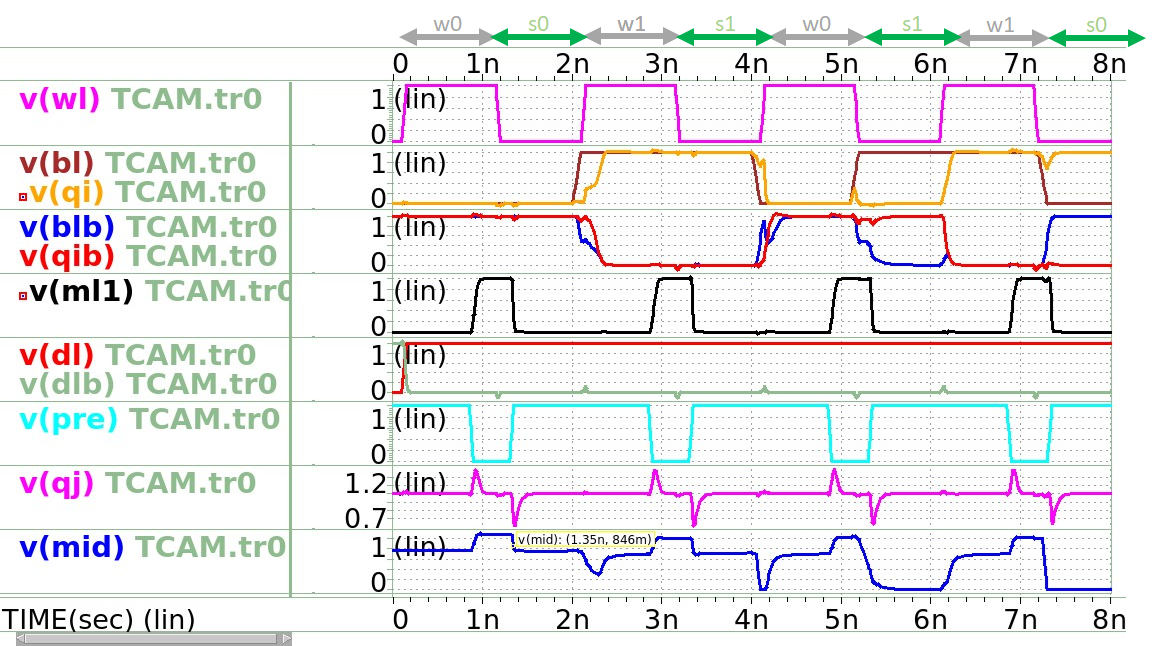
\includegraphics[width=\linewidth]{./img/2023-12-14-00-14-04.png}
\end{figure}

\clearpage

\section{NOR-type TCAM}

$\bullet$ Store Mode: WL 提升至 $V_{DD}$(1)。可以寫入 $BL$ 的值到 $Q_i$ , $\overline{BL}$ 的值到 $\overline{Q_i}$。

$\bullet$ Search Mode: 當 $Q_i = V_{DD},\ \overline{Q_i} = V_{DD}$ (storeX) 或 $\rm SL = 0,\ \overline{SL} = 0$ (sX),此為 Don't care mode。不管 $Q_i(\overline{Q_i})$ 和 $\rm SL(\overline{SL})$ 有沒有匹配。 ML 都 match (1(M))。反之,當不為 $Q_i = V_{DD},\ \overline{Q_i} = V_{DD}$ 且不為 $\rm SL = 0,\ \overline{SL} = 0$, 此為 Care mode,匹配資訊在下方。


\begin{table}[H]
  \centering
  \begin{tabular}{ccccc}
  $Q_i$ & $\overline{Q_i}$& $\rm SL$ & $\rm \overline{SL}$ & ML \\
  0  & 1     & 0  & 1     & 1(M) \\
  0  & 1     & 1  & 0     & 0(MM) \\
  1  & 0     & 0  & 1     & 0(MM) \\
  1  & 0     & 1  & 0     & 1(M) \\

  \end{tabular}
  \end{table}

  \begin{figure}[H]
    \centering
    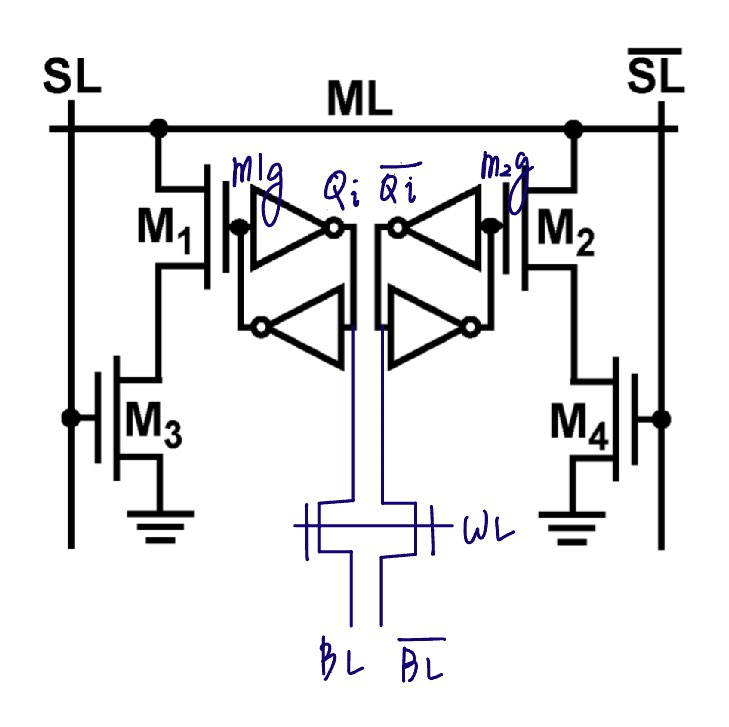
\includegraphics[width=0.7\linewidth]{./img/2023-12-14-00-36-36.png}
    \caption{NOR-type Circuit}
    \end{figure}


\subsection{Store Mode}

WL 電壓提升至 $V_{DD}$ 為 logic-1, 將兩個 nMOS 打開,即可用 $\rm BL$ 和 $\rm \overline{BL}$ 寫入資料到 $Q_i$ 和 $\overline{Q_i}$。圖上方的 w0 為寫入 $Q_i = 0$, $\overline{Q_i} = 1$, w1 為寫入 $Q_i = 1$, $\overline{Q_i} = 0$,wX 為寫入 $Q_i = 1$, $\overline{Q_i} = 1$。


\begin{figure}[H]
\centering
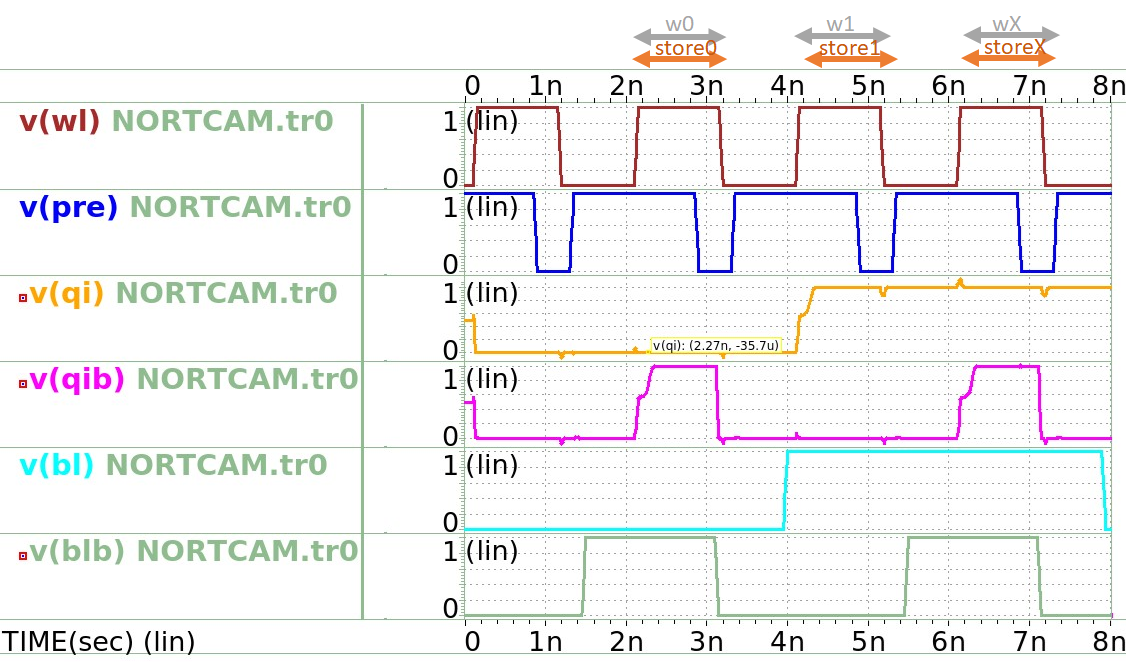
\includegraphics[width=\linewidth]{./img/2023-12-14-00-04-36.png}
\end{figure}


\subsection{Search Mode - Care mode}

在 Care mode 下,不要儲存 $Q_i = V_{DD},\ \overline{Q_i} = V_{DD}$ (storeX) 且不要搜索線為 $\rm SL = 0,\ \overline{SL} = 0$ (sX),以確保此電路在 Care Mode 下操作
。w為寫入,s為搜索資料。match (M) 為 1,mismatch (MM) 為 0。



\begin{figure}[H]
  \centering
  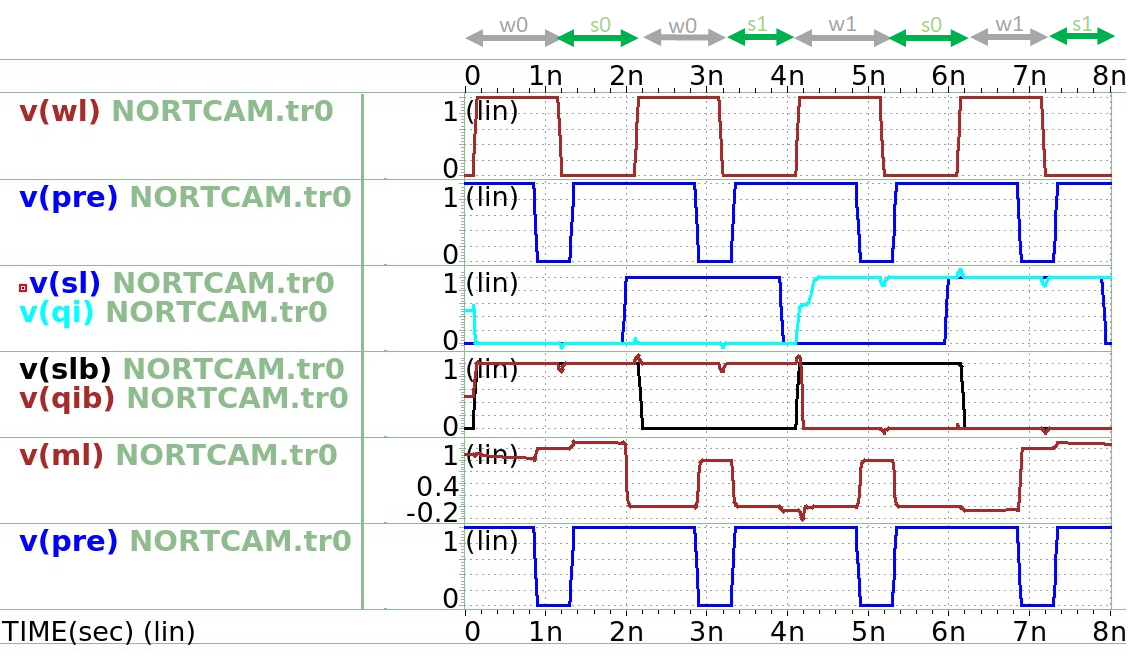
\includegraphics[width=\linewidth]{./img/2023-12-14-00-20-00.png}
  \end{figure}


\subsection{Search Mode - Don't care mode for storeX ($\bf Q_i = 1\ \&\ \overline{Q_i} = 1$)}

在 Don't Care mode 下, $Q_i = V_{DD},\ \overline{Q_i} = V_{DD}$,以確保此電路在 Don't Care Mode 下操作。
不管 $\rm SL$ 和 $\rm \overline{SL}$ 給值如何,都 Match (M) 為 VDD(1)。
w為寫入,s為搜索資料。

\begin{table}[H]
  \centering
  \begin{tabular}{ccccc}
  $Q_i$ & $\overline{Q_i}$& $\rm SL$ & $\rm \overline{SL}$ & ML \\
  1  & 1     & 0  & 1     & 1(M) \\
  1  & 1     & 0  & 0     & 1(M) \\
  1  & 1     & 1  & 1     & 1(M) \\
  1  & 1     & 1  & 0     & 1(M) \\
 
  \end{tabular}
  \end{table}


\begin{figure}[H]
\centering
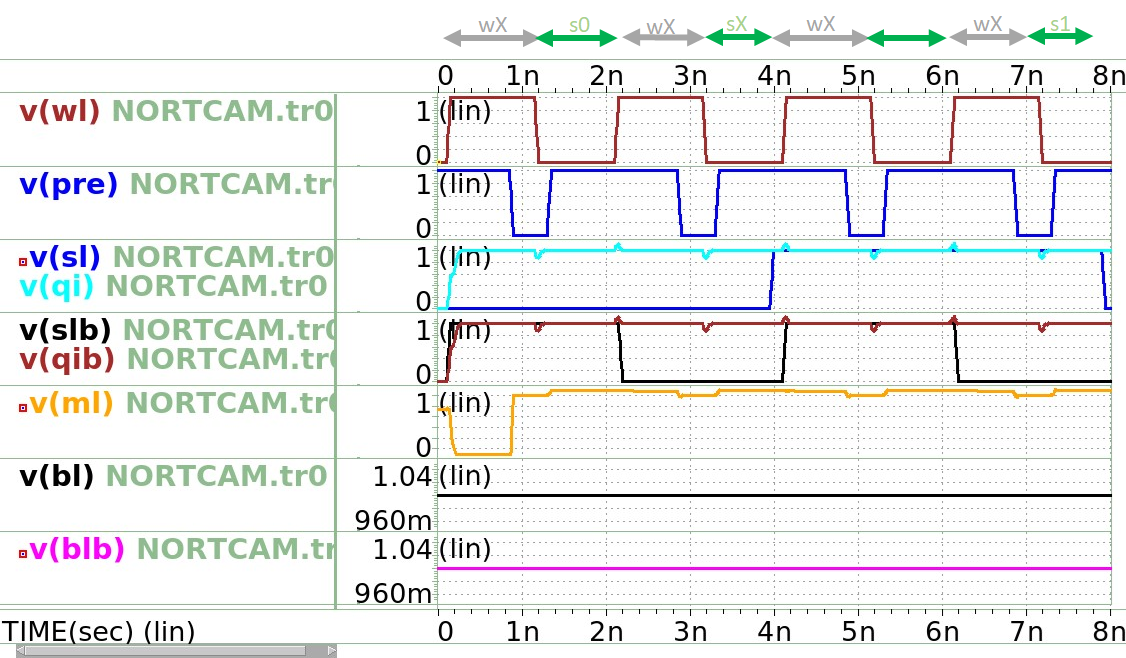
\includegraphics[width=\linewidth]{./img/2023-12-14-07-35-29.png}
\end{figure}

\subsection{Search Mode - Don't care mode for searchX ($\bf SL = 0\ \& \ \overline{SL} = 0$)}

在 Don't Care mode 下, $\rm SL = 0,\ \overline{SL} = 0$,以確保此電路在 Don't Care Mode 下操作。
不管 $Q_i$ 和 $\overline{Q_i}$ 給值如何,都 Match (M) 為 VDD(1)。
w為寫入,s為搜索資料。

\begin{table}[H]
  \centering
  \begin{tabular}{ccccc}
  $Q_i$ & $\overline{Q_i}$& $\rm SL$ & $\rm \overline{SL}$ & ML \\
  0  & 1     & 0  & 0     & 1(M) \\
  0  & 0     & 0  & 0     & 1(M) \\
  1  & 1     & 0  & 0     & 1(M) \\
  1  & 0     & 0  & 0     & 1(M) \\
 
  \end{tabular}
  \end{table}


\begin{figure}[H]
  \centering
  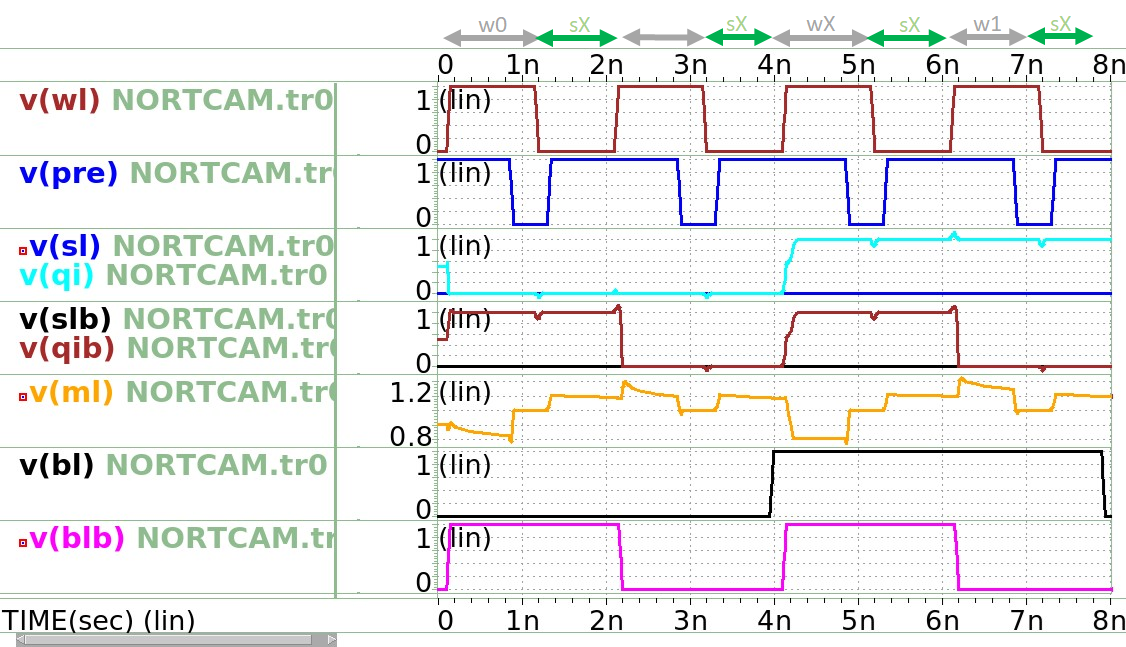
\includegraphics[width=\linewidth]{./img/2023-12-14-07-37-46.png}
  \end{figure}


  \section{參考資料}

  \begin{enumerate}
  
  \item\href{https://www.twblogs.net/a/5efe119e9644181341a1470a}{三態內容尋址存儲器(TCAM)工作原理}
  \item\href{http://103.82.172.44:8080/xmlui/bitstream/handle/123456789/28/A%20review%20of%20energy%20efficient%20ternary%20content%20.pdf?sequence=1&isAllowed=y&fbclid=IwAR1BU996txL15ISYrxkESIV1MQAB6pPLOH_FBdmN2Md4_hbKFK63faACwHc}{A review of energy efficient ternary content
  addressable memory (TCAM) circuits for network
  application}

\end{enumerate}

\end{document}